\chapter{Experimental Results}
\label{chap:Experimental Results}

\section{Evaluation Metrics}
To evaluate the performance of the forecasting model, several quantitative metrics are used. These metrics measure the difference between the temperature fields predicted by the neural network and the corresponding ground truth observations extracted from the ERA5 dataset.
The main evaluation metrics used in this project are the following.
\subsection{Mean Squared Error (MSE)}
The Mean Squared Error (MSE) measures the average squared difference between predicted values and observed values.
The formula can be written as:

MSE = (1 / N) × Σ (true value − predicted value)²

True value represents the real temperature value from the dataset, predicted value represents the temperature predicted by the model and N is the total number of observations.
This metric is used as the training loss function for the neural network. Minimizing the MSE encourages the model to produce predictions that are close to the real temperature fields.

\subsection{Root Mean Squared Error (RMSE)}
The Root Mean Squared Error (RMSE) is derived from the MSE and represents the square root of the mean squared error.
The formula is:
RMSE = √MSE
Unlike MSE, RMSE is expressed in the same unit as the predicted variable (Kelvin for temperature). This makes it easier to interpret the magnitude of prediction errors.
RMSE is particularly useful for comparing model performance across different forecast horizons.

\subsection{Mean Absolute Error (MAE)}
In addition to RMSE, the Mean Absolute Error (MAE) is also used to evaluate the accuracy of the predictions.
MAE measures the average absolute difference between predicted and true values:

MAE = average of |true value − predicted value|

Unlike MSE, MAE is less sensitive to large errors, which makes it useful for understanding the typical magnitude of prediction errors.

\section{Visualization}
Visual analysis of the results plays an important role in understanding the behavior of the forecasting model. Several visualizations are produced to evaluate both the training process and the quality of the generated forecasts.

\subsection{Training process}
The evolution of the training and validation losses is shown in Figure~\ref{fig:training_curves}.

\begin{figure}[h]
	\includegraphics[scale=0.6]{imagenes/Training_U_Net_version_française.pdf}
	\caption{Learning curves of the U-Net model trained using the Mean Squared Error (MSE) loss function.}
	\label{fig:training_curves}
\end{figure}

In Figure~\ref{fig:training_curves}, the blue curve corresponds to the training loss, while the orange curve represents the validation loss for the prediction at $t+6$ hours. Both curves exhibit a general decreasing trend throughout training, indicating that the neural network progressively learns to approximate the relationship between the atmospheric state at time $t$ and the state at $t+6$. Furthermore, the validation loss closely follows the training loss, suggesting that the model generalizes reasonably well to unseen data.

\subsection{Example of temperature prediction}
To qualitatively evaluate the model predictions, temperature maps generated by the model are compared with the corresponding ground truth observations, as illustrated in Figure~\ref{fig:temperature_comparison}.

\begin{figure}[h]
	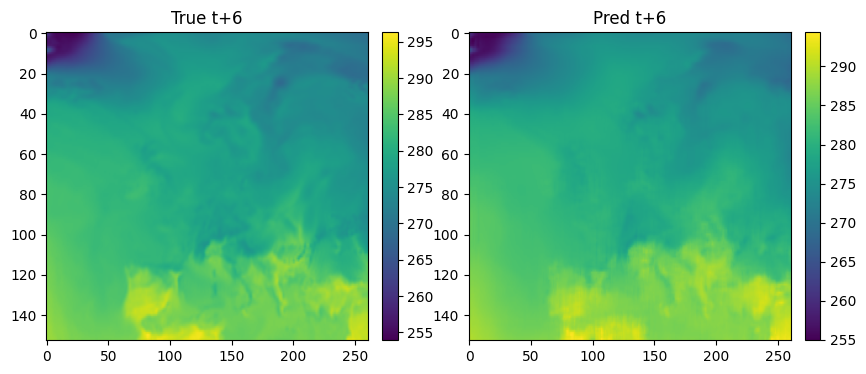
\includegraphics[scale=0.5]{imagenes/comparaison_réalité_prédiciton_version_française.png}
	\caption{Spatial field comparison between ground truth (left) and model prediction (right) at lead time t+6.}
	\label{fig:temperature_comparison}
\end{figure}

Both maps in Figure~\ref{fig:temperature_comparison} display the spatial distribution of temperature over the selected European region. The predicted map successfully reproduces the large-scale temperature patterns visible in the ground truth data. Major spatial structures, such as temperature gradients between northern and southern regions, are captured by the model.
Although some local differences remain, the predicted field preserves the overall structure of the atmospheric temperature distribution, indicating that the model has learned meaningful spatial representations.

\section{Forecast accuracy over multiple days}
To analyze how prediction accuracy evolves as the forecast horizon increases, recursive forecasting is performed using the trained model. In this framework, the model first generates a prediction for the next time step (e.g., $t+6$ hours), which is then fed back as input to predict the subsequent time step ($t+12$ hours). This iterative process is repeated multiple times, allowing the model to produce forecasts several days ahead. While this approach enables long-range predictions without requiring additional input data, it also introduces the accumulation of errors over time, as inaccuracies in earlier predictions can propagate and amplify in later steps.

\begin{figure}[h]
	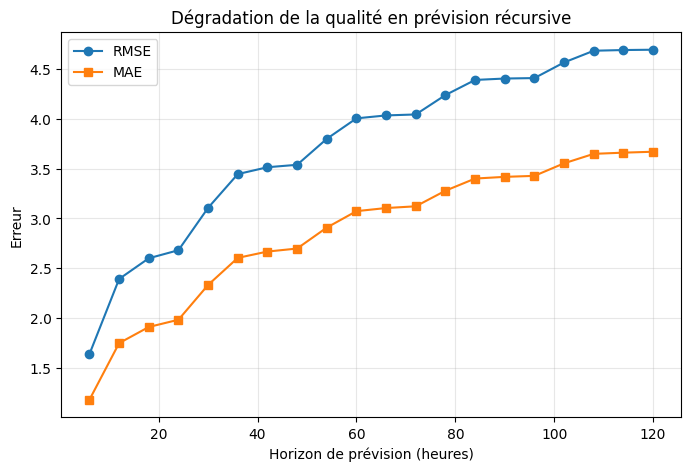
\includegraphics[scale=0.6]{imagenes/dégradation_mesure_version_française.png}
	\caption{Evolution of RMSE and MAE as a function of forecast lead time.}
	\label{fig:error_degradation}
\end{figure}

Figure~\ref{fig:error_degradation} illustrates the evolution of RMSE and MAE as a function of forecast lead time. Several observations can be made from this graph:
\begin{itemize}
	\item Prediction errors increase as the forecast horizon becomes larger.
	\item The model achieves the lowest error for short-term forecasts (around 6 hours).
	\item As predictions extend to multiple days ahead, the error gradually increases due to the accumulation of uncertainty in recursive predictions.
\end{itemize}

This behavior, clearly visible in Figure~\ref{fig:error_degradation}, is consistent with typical weather forecasting systems, where short-term predictions are generally more accurate than long-range forecasts.
Overall, the results demonstrate that the neural network is capable of producing reasonable short-term temperature forecasts and capturing important spatial structures in atmospheric data.